\newpage
\section{Theory of the Fourier Transform of the Fast Rotation Signal}

\subsection{Mathematical Preliminaries}

\begin{definition}[Fourier's transform and inverse transform]
Given a function $f$, its Fourier transform is \[\hat{f}(x)=\frac{1}{\sqrt{2\pi}}\int^{\infty}_{-\infty}f(t)e^{ixt}dt\] and its inverse Fourier transform is \[\tilde{f}(x)=\frac{1}{\sqrt{2\pi}}\int^{\infty}_{-\infty}f(t)e^{-ixt}dt\] If $f$ is absolutely integrable, then the Fourier transforms of $f$ always exist. It is easy to check that $f=\tilde{\hat{f}}=\hat{\tilde{f}}$.
\end{definition}

\begin{theorem}[Fourier's Integral]
For any piecewise continuous, piecewise differentiable, and absolutely integrable function $f$, the following equality holds: \[f(x)=\frac{1}{\pi}\int^{\infty}_0d\omega\int^{\infty}_{-\infty}f(t)\cos\omega(t-x)dt\]
\end{theorem}

If $f$ is even, then Fourier's integral simplifies to \[f(x)=\frac{2}{\pi}\int^{\infty}_0\cos\omega xd\omega\int^{\infty}_0f(t)\cos\omega tdt\]Suppose $f$ is a piecewise continuous, piecewise differentiable, and absolutely integrable function on $[0,\infty)$. If we extend $f$ to an even function defined on the whole real line, then the formula above is valid for the extension. In particular, it is also valid for $x\geq 0$.

\begin{theorem}[Convolution Theorem]
The convolution of two functions $f$ and $g$ is defined to be \[(f\ast g)(t)=\frac{1}{\sqrt{2\pi}}\int^{\infty}_{-\infty}f(\tau)g(t-\tau)d\tau\] The convolution theorem states that \[\widehat{f\ast g}=\hat{f}\hat{g} \text{ and } \widetilde{f\ast g}=\tilde{f}\tilde{g}\] 
\end{theorem}

%Suppose the supports of $f$ and $g$ are $(t_1,t_2)$ and $(t_3,t_4)$, respectively. Then \[(f\ast g)(t)=\int^{\infty}_{-\infty}f(\tau)g(t-\tau)d\tau=\int^{t_2}_{t_1}f(\tau)g(t-\tau)d\tau\] As $\tau$ increases from $t_1$ to $t_2$, the argument of $g(t-\tau)$ decreases from $t-t_1$ to $t-t_2$. Therefore the integrand vanishes if $t$ is such that $t-t_1<t_3$ or $t-t_2>t_4$. Hence the support of $(f\ast g)(t)$ is $(t_1+t_3,t_2+t_4)$.%

\subsection{The case of initially zero bunch length}

In this case we have that $\xi(t')=\delta(t')$, so the fast rotation signal becomes \[S(t)=\sum^{\infty}_{n=0}\frac{\rho\left(\frac{t}{(n+\theta/2\pi)T}-1\right)}{(n+\theta/2\pi)T}\]
Assuming the bunch evolves such that in the first turn the beam spreads negligibly, the center of mass of the bunch reaches the fiber harp at position $\theta$ at some time $t_0$. This $t_0$ is the time when muons at the magic frequency first reach the detector. Furthermore, we have that $\theta/2\pi=t_0/T$, so we may write 

\[
S(t)=\sum^{\infty}_{n=0}\frac{\rho\left(\frac{t}{nT+t_0}-1\right)}{nT+t_0}
\]
We next assume that $\mathcal{S}(t)\equiv S(t+t_0)$ is sufficiently well behaved so as to be absolutely integrable on $[0,\infty)$, as well as piecewise continuous and piecewise differentiable. Note that this means that $\rho(\Delta)$ must satisfy these conditions also. Extend $\mathcal{S}$ to the entire real line as an even function. By Theorem 1, we may express $\mathcal{S}$ as \[\mathcal{S}(t)=\frac{2}{\pi}\int^{\infty}_0\cos\omega td\omega\int^{\infty}_0\mathcal{S}(t')\cos\omega t'dt'\] We then recover $S(t)$:\[S(t+t_0)=\frac{2}{\pi}\int^{\infty}_0\cos\omega td\omega\int^{\infty}_0S(t'+t_0)\cos\omega t'dt'=\]\[\frac{2}{\pi}\int^{\infty}_0\cos\omega td\omega\int^{\infty}_{t_0}S(t')\cos\omega(t'-t_0)dt'\Rightarrow\]

\[
S(t)=\frac{2}{\pi}\int^{\infty}_0\cos\omega(t-t_0)d\omega\int^{\infty}_{t_0}S(t')\cos\omega(t'-t_0)dt'
\] 
But we also know from Definition 1 that \[\mathcal{S}(t)=\tilde{\hat{\mathcal{S}}}(t)=\frac{1}{2\pi}\int^{\infty}_{-\infty}e^{-i\omega t}d\omega\int^{\infty}_{-\infty}\mathcal{S}(t')e^{i\omega t'}dt'=\]\[\frac{1}{2\pi}\int^{\infty}_{-\infty}e^{-i\omega t}d\omega\int^{\infty}_{-\infty}\mathcal{S}(t')(\cos\omega t'+i\sin\omega t')dt'=\frac{1}{2\pi}\int^{\infty}_{-\infty}e^{-i\omega t}d\omega\int^{\infty}_{-\infty}\mathcal{S}(t')\cos\omega t'dt'\] where we used the fact that $\mathcal{S}$ is an even function, and the integral of the product of an even and odd function vanishes. From the preceding expression we now see that $\hat{\mathcal{S}}$ is an even function. So we write \[\frac{1}{2\pi}\int^{\infty}_{-\infty}\hat{\mathcal{S}}(\omega)\cos\omega td\omega=\frac{1}{\pi}\int^{\infty}_0\hat{\mathcal{S}}(\omega)\cos\omega td\omega=\frac{2}{\pi}\int^{\infty}_0\cos\omega td\omega\int^{\infty}_0\mathcal{S}(t')\cos\omega t'dt'\] Thus 

\begin{equation}
\hat{S}(\omega)=\sqrt{\frac{2}{\pi}}\int^{\infty}_{t_0}S(t)\cos\omega(t-t_0)dt
\label{eq:nospreadFT}
\end{equation} 
is the Fourier transform of $S$. So if we're given $\hat{S}(\omega)$, we may express $S$ as 

\begin{equation}
S(t)=\sqrt{\frac{2}{\pi}}\int^{\infty}_0\hat{S}(\omega)\cos\omega(t-t_0)d\omega=\frac{1}{\sqrt{2\pi}}\int^{\infty}_{-\infty}\hat{S}(\omega)\cos\omega(t-t_0)d\omega
\label{eq:nospreadIFT}
\end{equation}

\subsection{Bunch Length Distribution $\xi(t')$}
We call the fast rotation signal with no inital bunch length $S_0(t)$. Given an initial longitudinal distribution $\xi(t')$, the fast rotation signal is described by \[S(t)=\int\xi(t')S_0(t-t')dt'=\sqrt{2\pi}(\xi\ast S_0)(t)\] In the ideal case we would directly apply the convolution theorem to find that 

\begin{equation}
\hat{S}(\omega)=\sqrt{2\pi}\hat{\xi}(\omega)\hat{S}_0(\omega)
\label{eq:ConvoSpectrum}
\end{equation} However, we won't have $S_0(t)$ to work with directly, nor $\xi(t)$. We need to use $S(t)$ to get $\hat{S}(\omega)$. 

We express $S_0(t-t')$ through Fourier's integral: \[S_0(t-t')=\frac{2}{\pi}\int^{\infty}_0\cos\omega(t-t_0-t')d\omega\int^{\infty}_{t_0}S_0(\bar{t})\cos\omega(\bar{t}-t_0)d\bar{t}=\]\[\sqrt{\frac{2}{\pi}}\int^{\infty}_0\hat{S}_0(\omega)\cos\omega(t-t_0-t')d\omega\] Substituting this expression into the convolution integral, we get \[S(t)=(\xi\ast S_0)(t)=\int^{\infty}_{-\infty}\xi(t)S_0(t-t')dt'=\sqrt{\frac{2}{\pi}}\int^{\infty}_0\hat{S}_0(\omega)d\omega\int^{\infty}_{-\infty}\xi(t')\cos\omega(t-t_0-t')dt'=\]\[\sqrt{\frac{2}{\pi}}\int^{\infty}_0\hat{S}_0(\omega)\langle\cos\omega(t-t_0-t')\rangle d\omega=\]\[\sqrt{\frac{2}{\pi}}\int^{\infty}_0\hat{S}_0(\omega)\langle\cos\omega(t-t_0)\cos\omega t'+\sin\omega(t-t_0)\sin\omega t'\rangle d\omega=\]\[\sqrt{\frac{2}{\pi}}\left(\int^{\infty}_0\hat{S}_0(\omega)\langle\cos\omega t'\rangle\cos\omega(t-t_0)d\omega+\int^{\infty}_0\hat{S}_0(\omega)\langle\sin\omega t'\rangle\sin\omega(t-t_0)d\omega\right)\] where $\langle\text{ }\rangle$ denotes averaging with respect to $\xi(t)$. 

If $\xi(t')$ is even, $\langle\sin\omega t'\rangle=0$. We are then left with 

\begin{equation}
S(t)=\sqrt{\frac{2}{\pi}}\int^{\infty}_0\hat{S}_0(\omega)\langle\cos\omega t'\rangle\cos\omega(t-t_0)d\omega
\label{eq:EvenBunchFT}
\end{equation} suggesting that $\hat{S}(\omega)=\hat{S}_0(\omega)\langle\cos\omega t'\rangle$. We can see that this is true by looking back at$~\eqref{eq:ConvoSpectrum}$: \[\hat{\xi}(\omega)=\frac{1}{\sqrt{2\pi}}\int^{\infty}_{-\infty}\xi(t')e^{i\omega t'}dt'=\frac{1}{\sqrt{2\pi}}\int^{\infty}_{-\infty}\xi(t')\cos\omega t'dt'=\frac{\langle\cos\omega t'\rangle}{\sqrt{2\pi}}\] and therefore $\hat{S}(\omega)=\sqrt{2\pi}\hat{\xi}(\omega)\hat{S}_0(\omega)=\hat{S}_0(\omega)\langle\cos\omega t'\rangle$. Thus$~\eqref{eq:EvenBunchFT}$ is the inverse Fourier transform, implying that 

\begin{equation}
\hat{S}(\omega)=\sqrt{\frac{2}{\pi}}\int^{\infty}_{t_0}S(t)\cos\omega(t-t_0)dt
\label{eq:integEvenBunchFT}
\end{equation}

If $\xi(t')$ is not symmetric, then we are faced with the problem that $\hat{S}(\omega)$ features an imaginary component.

\subsection{Corrections to the Fourier Transform}

If the detector detects the muons at a time $t_s>t_0$, then the resulting Fourier transform of the observed fast rotation signal has a missing component 
\begin{equation}
\Delta(\omega)=\sqrt{\frac{2}{\pi}}\int^{t_s}_{t_0}S(t)\cos\omega(t-t_0)dt
\label{eq:Delta}
\end{equation} while the immediately observed frequency spectrum is 

\begin{equation}
\hat{S}(\omega)=\sqrt{\frac{2}{\pi}}\int^{\infty}_{t_s}S(t)\cos\omega(t-t_0)dt
\label{eq:firstapprox}
\end{equation}
However, we do not observe $S(t)$ on $(t_0,t_s)$, so we need to find a way to correct the frequency spectrum. 

In order to do this, we first note that the Fourier transform has associated with it an uncertainty principle, namely that $\Delta f\Delta t\sim1$. If $t_s$ isn't too great, we can then expect that the spread of $\Delta(\omega)$ about the magic frequency will be large while the spread of $\hat{S}(\omega)$ will change negligibly. So we may express $S(t)$ using the observed $\hat{S}(\omega)$ through formula$~\eqref{eq:nospreadIFT}$. Thus we have that \[\Delta(\omega)=\frac{2}{\pi}\int^{t_s}_{t_0}\int^{\infty}_0\hat{S}(\omega')\cos\omega'(t-t_0)\cos\omega(t-t_0)d\omega' dt\] Integrating with respect to $t$ first, we get \[\Delta(\omega)=\frac{1}{\pi}\int^{\infty}_0\hat{S}(\omega)\left(\frac{\sin(\omega-\omega')(t_s-t_0)}{\omega-\omega'}+\frac{\sin(\omega+\omega')(t_s-t_0)}{\omega+\omega'}\right)d\omega'\] We may neglect the second term in the parentheses, as we are interested in frequencies $\omega$ such that $|\omega-\omega'|<<\omega+\omega'$, so 

\begin{equation}
\Delta(\omega)=\frac{1}{\pi}\int^{\infty}_0\hat{S}(\omega)\frac{\sin(\omega-\omega')(t_s-t_0)}{\omega-\omega'}d\omega'
\label{eq:approxDelta}
\end{equation}

\subsection{Physical Interpretation of the Fourier Transform of the Fast Rotation Signal}

Assuming that the energy offset distribution $\rho(\Delta)$ is centered with a maximum at $\Delta=0$, the harmonics of the Fourier transform of the fast rotation signal will be featured at integer multiples of the magic frequency; this is evident from the construction of the general fast rotation signal. The signal is due to the orbits of muons at various revolution frequencies, so $\hat{S}(\omega)$ describes the distribution of revolution frequencies among the muons. However, the muons are restricted to the vacuum chamber, making frequencies corresponding to muons outside the chamber nonphysical. Hence the first harmonic corresponds to the physical revolution frequency distribution of the muons.

\section{Analysis for a Gaussian Energy Offset Distribution and Initially Zero Bunch Length}

If the energy offset distribution is a Gaussian with width $\Delta_0$, then \[S(t)=\sum^{\infty}_{n=0}\frac{e^{-(t-(nT+t_0))^2/2\Delta^2_0(nT+t_0)^2}}{\sqrt{2\pi}\Delta_0(nT+t_0)}\] Suppose the center of mass of the muon beam first passes the detector at time $t_0$, and the detector starts detecting at some time $t_s>t_0$. Then the Fourier transform of the fast rotation signal is

\begin{gather}
\hat{S}(\omega)=\sqrt{\frac{2}{\pi}}\int^{\infty}_{t_s}S(t)\cos\omega(t-t_0) dt \nonumber \\
=\sqrt{\frac{2}{\pi}}\sum^{\infty}_{n=0}\int^{\infty}_{t_s}\frac{e^{-(t-(nT+t_0))^2/2\Delta^2_0(nT+t_0)^2}}{\sqrt{2\pi}\Delta_0(nT+t_0)}\cos\omega(t-t_0)dt \nonumber \\ 
=\sqrt{\frac{2}{\pi}}\sum^{\infty}_{n=0}\frac{e^{-1/2\Delta^2_0}}{2\sqrt{2\pi}\Delta_0(nT+t_0)}\int^{\infty}_{t_s}e^{-t^2/2\Delta^2_0(nT+t_0)^2}e^{t/(nT+t_0)\Delta^2_0}e^{\pm i\omega t}e^{\mp i\omega t_0}dt.
\end{gather}

From Gradshteyn and Rizhik, we know that 
\begin{equation}
\int^{\infty}_u\exp\left(-\frac{x^2}{4\beta}-\gamma x\right)dx=\sqrt{\pi\beta}e^{\beta\gamma^2}\left(1-\frac{\sqrt{\pi}}{2}\text{Erf}\left(\gamma\sqrt{\beta}+\frac{u}{2\sqrt{\beta}}\right)\right)
\label{eq:GradRyzhik}
\end{equation}
for $\text{Re}(\beta)>0$ and $u\geq0$. Thus the result of using this integral in computing the Fourier transform is $\hat{S}(\omega)=$ 

\begin{gather}
\sqrt{\frac{2}{\pi}}\sum^{\infty}_{n=0}\frac{e^{-\omega^2(nT+t_0)^2\Delta^2_0/2}e^{i\omega nT}}{4}\left(1-\frac{\sqrt{\pi}}{2}\text{Erf}\left[\frac{-1}{\Delta_0\sqrt{2}}-\frac{i\omega (nT+t_0)\Delta_0}{\sqrt{2}}+\frac{t_s}{\Delta_0(nT+t_0)\sqrt{2}}\right]\right)+ \nonumber \\
\sqrt{\frac{2}{\pi}}\sum^{\infty}_{n=0}\frac{e^{-\omega^2(nT+t_0)^2\Delta^2_0/2}e^{-i\omega nT}}{4}\left(1-\frac{\sqrt{\pi}}{2}\text{Erf}\left[\frac{-1}{\Delta_0\sqrt{2}}+\frac{i\omega (nT+t_0)\Delta_0}{\sqrt{2}}+\frac{t_s}{\Delta_0(nT+t_0)\sqrt{2}}\right]\right)
\end{gather}

\subsection{Corrections to the Fourier transform} The detector in the section above started to detect the muon beam at a time $t_s>t_0$. This results in some lost frequency content in the Fourier transform above, creating distortions of the frequency spectrum. The missing part of the frequency spectrum is described by formula$~\eqref{eq:Delta}$. Let's take a closer look at $\Delta$. \[\Delta(\omega)=\sqrt{\frac{2}{\pi}}\int^{t_s}_{t_0}S(t)\cos\omega(t-t_0)dt\]\[=\sqrt{\frac{2}{\pi}}\int^{\infty}_{t_0}S(t)\cos\omega(t-t_0)dt-\sqrt{\frac{2}{\pi}}\int^{\infty}_{t_s}S(t)\cos\omega(t-t_0)dt\] Using$~\eqref{eq:GradRyzhik}$, we have 

\begin{gather}
\sqrt{\frac{2}{\pi}}\sum^{\infty}_{n=0}\frac{e^{-\omega^2(nT+t_0)^2\Delta^2_0/2}e^{i\omega nT}}{4}\left(1-\frac{\sqrt{\pi}}{2}\text{Erf}\left[\frac{-1}{\Delta_0\sqrt{2}}-\frac{i\omega (nT+t_0)\Delta_0}{\sqrt{2}}+\frac{t_0}{\Delta_0(nT+t_0)\sqrt{2}}\right]\right)+ \nonumber \\
\sqrt{\frac{2}{\pi}}\sum^{\infty}_{n=0}\frac{e^{-\omega^2(nT+t_0)^2\Delta^2_0/2}e^{-i\omega nT}}{4}\left(1-\frac{\sqrt{\pi}}{2}\text{Erf}\left[\frac{-1}{\Delta_0\sqrt{2}}+\frac{i\omega (nT+t_0)\Delta_0}{\sqrt{2}}+\frac{t_0}{\Delta_0(nT+t_0)\sqrt{2}}\right]\right) \nonumber \\
-\sqrt{\frac{2}{\pi}}\sum^{\infty}_{n=0}\frac{e^{-\omega^2(nT+t_0)^2\Delta^2_0/2}e^{i\omega nT}}{4}\left(1-\frac{\sqrt{\pi}}{2}\text{Erf}\left[\frac{-1}{\Delta_0\sqrt{2}}-\frac{i\omega (nT+t_0)\Delta_0}{\sqrt{2}}+\frac{t_s}{\Delta_0(nT+t_0)\sqrt{2}}\right]\right)+ \nonumber \\
-\sqrt{\frac{2}{\pi}}\sum^{\infty}_{n=0}\frac{e^{-\omega^2(nT+t_0)^2\Delta^2_0/2}e^{-i\omega nT}}{4}\left(1-\frac{\sqrt{\pi}}{2}\text{Erf}\left[\frac{-1}{\Delta_0\sqrt{2}}+\frac{i\omega (nT+t_0)\Delta_0}{\sqrt{2}}+\frac{t_s}{\Delta_0(nT+t_0)\sqrt{2}}\right]\right)
\end{gather}

\begin{figure}[bt]
\centering
\subfigure[]{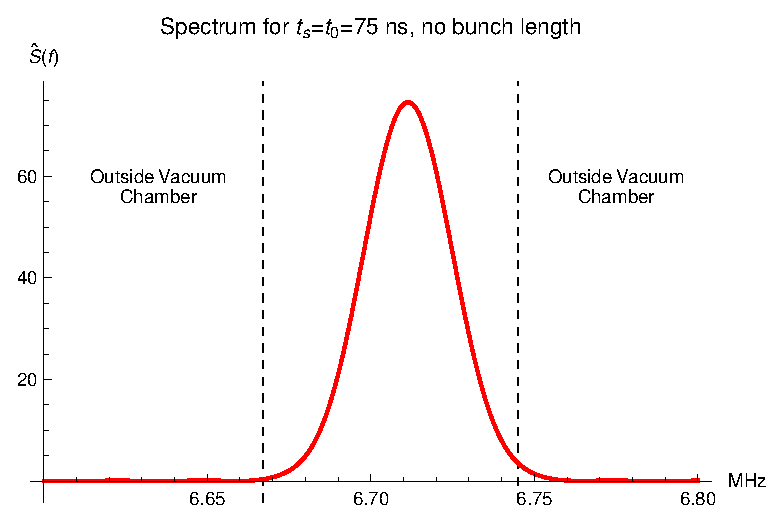
\includegraphics[scale=0.8]{fig/IdealFT_no_tspread.eps}}
\subfigure[]{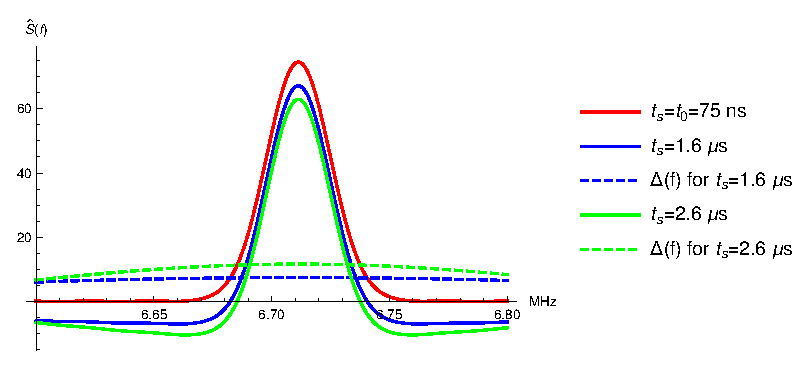
\includegraphics[scale=1.2]{fig/FT_no_tspread.eps}}
\caption{Frequency spectra for the case of a Gaussian energy offset distribution and no initial bunch length. Spectra for different $t_s$ are displayed, as well the corresponding $\Delta(f)$ functions}
\label{fig:FT_no_tspread}
\end{figure}

Figure~\ref{fig:FT_no_tspread} shows how the Fourier transform and the corresponding corrections are altered by increasing $t_s$.

\section{Analysis for a Gaussian Energy Offset Distribution and Gaussian Longitudinal Distribution}

The fast rotation signal in this case is of the same form as in the case of no longitudinal distribution: \[S(t)=\sum^{\infty}_{n=0}\frac{e^{-(t-(nT+t_0))^2/2\Delta'^2_0(nT+t_0)^2}}{\sqrt{2\pi}\Delta'_0(nT+t_0)}\] Thus $\hat{S}(\omega)=$ 

\begin{gather}
\sqrt{\frac{2}{\pi}}\sum^{\infty}_{n=0}\frac{e^{-\omega^2(nT+t_0)^2\Delta'^2_0/2}e^{i\omega nT}}{4}\left(1-\frac{\sqrt{\pi}}{2}\text{Erf}\left[\frac{-1}{\Delta'_0\sqrt{2}}-\frac{i\omega (nT+t_0)\Delta'_0}{\sqrt{2}}+\frac{t_s}{\Delta'_0(nT+t_0)\sqrt{2}}\right]\right)+ \nonumber \\
\sqrt{\frac{2}{\pi}}\sum^{\infty}_{n=0}\frac{e^{-\omega^2(nT+t_0)^2\Delta'^2_0/2}e^{-i\omega nT}}{4}\left(1-\frac{\sqrt{\pi}}{2}\text{Erf}\left[\frac{-1}{\Delta'_0\sqrt{2}}+\frac{i\omega (nT+t_0)\Delta'_0}{\sqrt{2}}+\frac{t_s}{\Delta'_0(nT+t_0)\sqrt{2}}\right]\right)
\end{gather}
and $\Delta(\omega)=$
\begin{gather}
\sqrt{\frac{2}{\pi}}\sum^{\infty}_{n=0}\frac{e^{-\omega^2(nT+t_0)^2\Delta'^2_0/2}e^{i\omega nT}}{4}\left(1-\frac{\sqrt{\pi}}{2}\text{Erf}\left[\frac{-1}{\Delta'_0\sqrt{2}}-\frac{i\omega (nT+t_0)\Delta'_0}{\sqrt{2}}+\frac{t_0}{\Delta'_0(nT+t_0)\sqrt{2}}\right]\right)+ \nonumber \\
\sqrt{\frac{2}{\pi}}\sum^{\infty}_{n=0}\frac{e^{-\omega^2(nT+t_0)^2\Delta'^2_0/2}e^{-i\omega nT}}{4}\left(1-\frac{\sqrt{\pi}}{2}\text{Erf}\left[\frac{-1}{\Delta_0\sqrt{2}}+\frac{i\omega (nT+t_0)\Delta'_0}{\sqrt{2}}+\frac{t_0}{\Delta'_0(nT+t_0)\sqrt{2}}\right]\right) \nonumber \\
-\sqrt{\frac{2}{\pi}}\sum^{\infty}_{n=0}\frac{e^{-\omega^2(nT+t_0)^2\Delta'^2_0/2}e^{i\omega nT}}{4}\left(1-\frac{\sqrt{\pi}}{2}\text{Erf}\left[\frac{-1}{\Delta_0\sqrt{2}}-\frac{i\omega (nT+t_0)\Delta'_0}{\sqrt{2}}+\frac{t_s}{\Delta'_0(nT+t_0)\sqrt{2}}\right]\right)+ \nonumber \\
-\sqrt{\frac{2}{\pi}}\sum^{\infty}_{n=0}\frac{e^{-\omega^2(nT+t_0)^2\Delta'^2_0/2}e^{-i\omega nT}}{4}\left(1-\frac{\sqrt{\pi}}{2}\text{Erf}\left[\frac{-1}{\Delta_0\sqrt{2}}+\frac{i\omega (nT+t_0)\Delta'_0}{\sqrt{2}}+\frac{t_s}{\Delta'_0(nT+t_0)\sqrt{2}}\right]\right)
\end{gather}

\begin{figure}[bt]
\centering
\subfigure[]{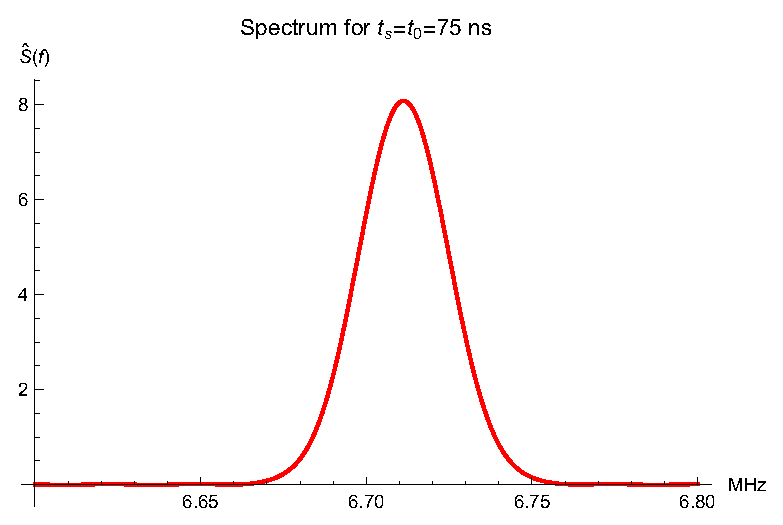
\includegraphics[scale=0.8]{fig/IdealFT_tspread.eps}}
\subfigure[]{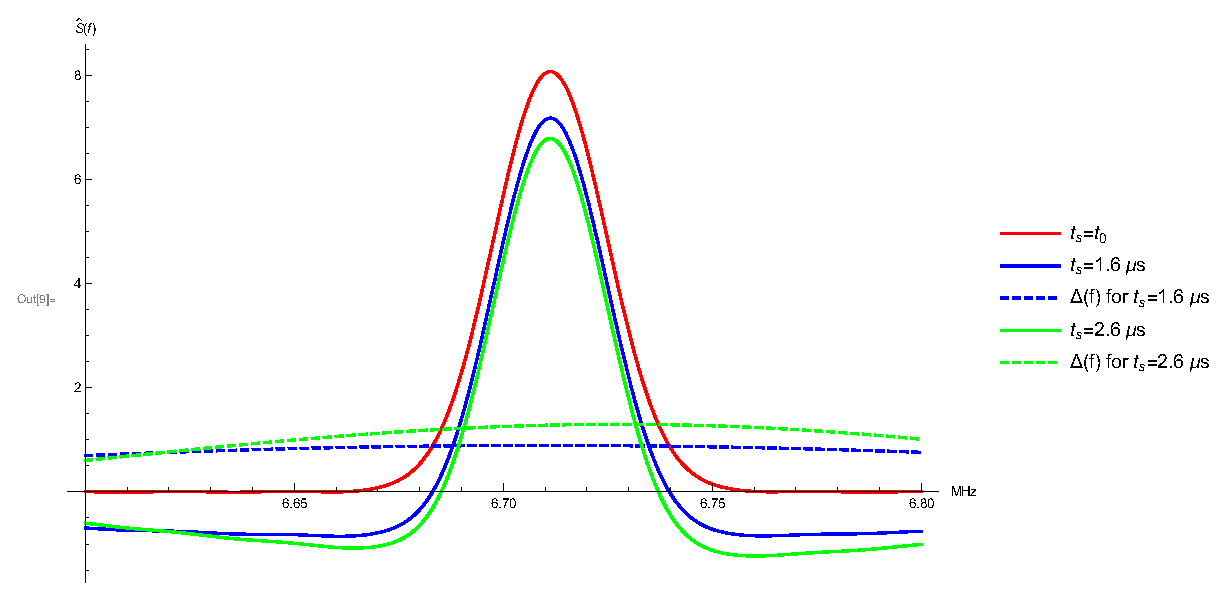
\includegraphics[scale=1.2]{fig/FT_tspread.eps}}
\caption{Frequency spectra for the case of a Gaussian energy offset distribution and Gaussian bunch length distribution. Spectra for different $t_s$ are displayed, as well the corresponding $\Delta(f)$ functions}
\label{fig:FT_tspread}
\end{figure}

Figure~\ref{fig:FT_tspread} shows how the Fourier transform and the corresponding corrections are altered by increasing $t_s$.
